\documentclass[11pt,a4paper]{article}

% -----------------------------------------------------------------------------
% Paquetes: todos forman parte de una instalacion estandar de LaTeX.
% -----------------------------------------------------------------------------
\usepackage[utf8]{inputenc}
\usepackage[T1]{fontenc}
\usepackage{amsmath, amssymb}
\usepackage{booktabs}
\usepackage{enumitem}
\usepackage{float} % Permite el uso del modificador de posicionamiento estricto [H]

% Fecha en espanol sin depender de babel ni de spanish.ldf.
\newcommand{\FechaEnEspanol}{%
  \number\day\space de\space
  \ifcase\month
    \or enero\or febrero\or marzo\or abril\or mayo\or junio\or
    julio\or agosto\or septiembre\or octubre\or noviembre\or diciembre
  \fi\space de\space\number\year
}
\usepackage[a4paper,margin=2.5cm,headheight=42pt]{geometry}
\usepackage{graphicx}
\usepackage{xcolor}
\usepackage{fancyhdr}

% lastpage no es necesario para compilar, pero permite mostrar "pagina de N".
\newif\ifHayUltimaPagina
\IfFileExists{lastpage.sty}{
  \usepackage{lastpage}
  \HayUltimaPaginatrue
}{
  \HayUltimaPaginafalse
}

% -----------------------------------------------------------------------------
% CONFIGURACION DEL TRABAJO
% -----------------------------------------------------------------------------
\newcommand{\NombreMateria}{Redes de Computadoras}
\newcommand{\TipoTrabajo}{Trabajo Práctico}
\newcommand{\NumeroTrabajo}{1}
\newcommand{\TipoTP}{Práctico}
\newcommand{\NombreTrabajo}{Laboratorio N\textsuperscript{o}1}
\newcommand{\NombreGrupo}{NetRunners}
\newcommand{\Docente}{Nombre y apellido del docente}
\newcommand{\LogoArchivo}{logo.png}
\newcommand{\LogoRuta}{\LogoArchivo}

\newcommand{\Integrantes}{%
  \begin{tabular}{ll}
    Bastida, Lucas Ramiro & DNI 39444511 \\
    Contessi, Ruben Andres & DNI 33315235 \\
    Garay, Ignacio Hernan & DNI 44191925 \\
    Giraudo, Juan Pablo & DNI 34970089 \\
    Peñaloza, Gonzalo Adrian & DNI 40441355 \\
    Quinteros del Castillo, Tomás Agustín & DNI 46169739 \\
    Vasconsellos Blason, Benjamin Alejandro & DNI 45642879 \\
  \end{tabular}%
}

% -----------------------------------------------------------------------------
% Elementos comunes de caratula y encabezado
% -----------------------------------------------------------------------------
\newcommand{\InsertarLogo}[1][0.24\textwidth]{%
  \ifx\LogoRuta\empty
    \fbox{\parbox[c][1cm][c]{#1}{\centering Logo institucional\\\small (colocar archivo)}}%
  \else
    \includegraphics[width=#1,keepaspectratio]{\LogoRuta}%
  \fi
}

\newcommand{\TituloCorto}{TP \NumeroTrabajo (\TipoTP): \NombreTrabajo}

\pagestyle{fancy}
\fancyhf{}
\fancyhead[L]{\InsertarLogo[1.4cm]}
\fancyhead[C]{\small\textbf{\TituloCorto}}
\fancyhead[R]{\small\NombreGrupo}
\renewcommand{\headrulewidth}{0.4pt}
\fancyfoot[C]{\small Pagina \thepage\ifHayUltimaPagina\ de \pageref{LastPage}\fi}
\renewcommand{\footrulewidth}{0pt}

\begin{document}

\begin{titlepage}
  \thispagestyle{empty}
  \begin{center}
    \InsertarLogo[0.32\textwidth]

    \vfill
    {\Large\textsc{\NombreMateria}\par}
    \vspace{1.5cm}
    {\Huge\bfseries \TipoTrabajo\par}
    \vspace{0.35cm}
    {\LARGE N.\textsuperscript{o} \NumeroTrabajo (\TipoTP)\par}
    \vspace{0.8cm}
    {\Large\NombreTrabajo\par}

    \vfill
    \begin{tabular}{rl}
      \textbf{Grupo:} & \NombreGrupo \\
      \textbf{Docente:} & \Docente
    \end{tabular}

    \vspace{1cm}
    \begin{center}
      \textbf{Integrantes}\\[0.2cm]
      \Integrantes
    \end{center}

    \vfill
    {\large \FechaEnEspanol\par}
  \end{center}
\end{titlepage}

\section{}

\begin{enumerate}[label=\alph*.]
    \setcounter{enumi}{1}
    \item Si consideramos que la onda viaja exactamente a la velocidad de la luz ($c = 3 \times 10^8 \text{ m/s}$) y usamos la relación $c = f \cdot \lambda$, analizando el gráfico vemos que un ciclo de onda corresponde a $60 \text{ mm}$. Teniendo la longitud de onda $\lambda$, la pasamos a metros:
    \[
    \lambda = 60 \text{ mm} = 0.06 \text{ m} = 6 \times 10^{-2} \text{ m}
    \]
    Despejando de la relación:
    \[
    f = \frac{c}{\lambda} = \frac{3 \times 10^8 \text{ m/s}}{0.06 \text{ m}} = 50 \times 10^8 \text{ Hz} = 5 \text{ GHz}
    \]

    \item Puntualmente, estos $5 \text{ GHz}$ se encuentran en la región entre $3 \text{ GHz}$ y $30 \text{ GHz}$, la cual corresponde a la banda \textbf{SHF} (\textit{Super High Frequency}), utilizando el espectro electromagnético y las definiciones de la ITU.

    \item En la banda SHF operan normalmente dispositivos comerciales de comunicación; evidentemente el más importante es el teléfono celular 5G, pero además los routers WiFi también operan en esta banda.

    \item Si observamos el gráfico, claramente el fenómeno que se presenta es el de \textbf{“Atenuación”}: observamos que la intensidad de la onda va disminuyendo a medida que aumenta la distancia.

    \item Tomando el ejemplo de los teléfonos celulares 5G, a medida que nos alejamos de las zonas urbanas donde se encuentran las grandes antenas de telefonía, notamos esta atenuación, hasta el punto de desaparecer.

    \item 
    \begin{enumerate}[label=\roman*)]
        \item Claramente sí, afecta a las transmisiones de telefonía celular, debido a que se mueve por un medio “no guiado” y depende de la distancia a las antenas y de la ubicación de los teléfonos celulares (si hay obstáculos, etc.).
        \item En las transmisiones por cable coaxial, al ser un medio guiado, al aumentar la distancia del cable empieza a aparecer la atenuación, e influye la frecuencia (a mayor frecuencia, mayor pérdida por metro de cable).
        \item Por último, en el caso de la fibra óptica la atenuación es mucho menor que en el cable coaxial debido a que en las transmisiones por cobre afectan efectos resistivos y pérdidas dieléctricas, mientras que en la fibra las pérdidas son más débiles ya que dependen de otros fenómenos.
    \end{enumerate}
\end{enumerate}

\section{}

\begin{enumerate}[label=\alph*.]
    \item Revisando la direccionalidad y las características, el gráfico hace referencia a una comunicación \textbf{Simplex síncrona}, es decir, un único sentido de los datos y con una señal de \textit{Clock} común entre emisor y receptor.

    \item Este paradigma no resulta útil si lo que queremos es una transmisión rápida y bidireccional; necesitaríamos adaptar el hardware (agregar otra línea, agregar más cableado y tener en cuenta pines extra, es decir, existe un \textit{trade-off} muy grande).

    \item La cuarta letra del nombre de nuestro grupo (\textbf{NetRunners}) es la \textbf{R}. Teniendo en cuenta el código ASCII, su representación binaria es \texttt{01010010}.
    
    \begin{figure}[H]
        \centering
        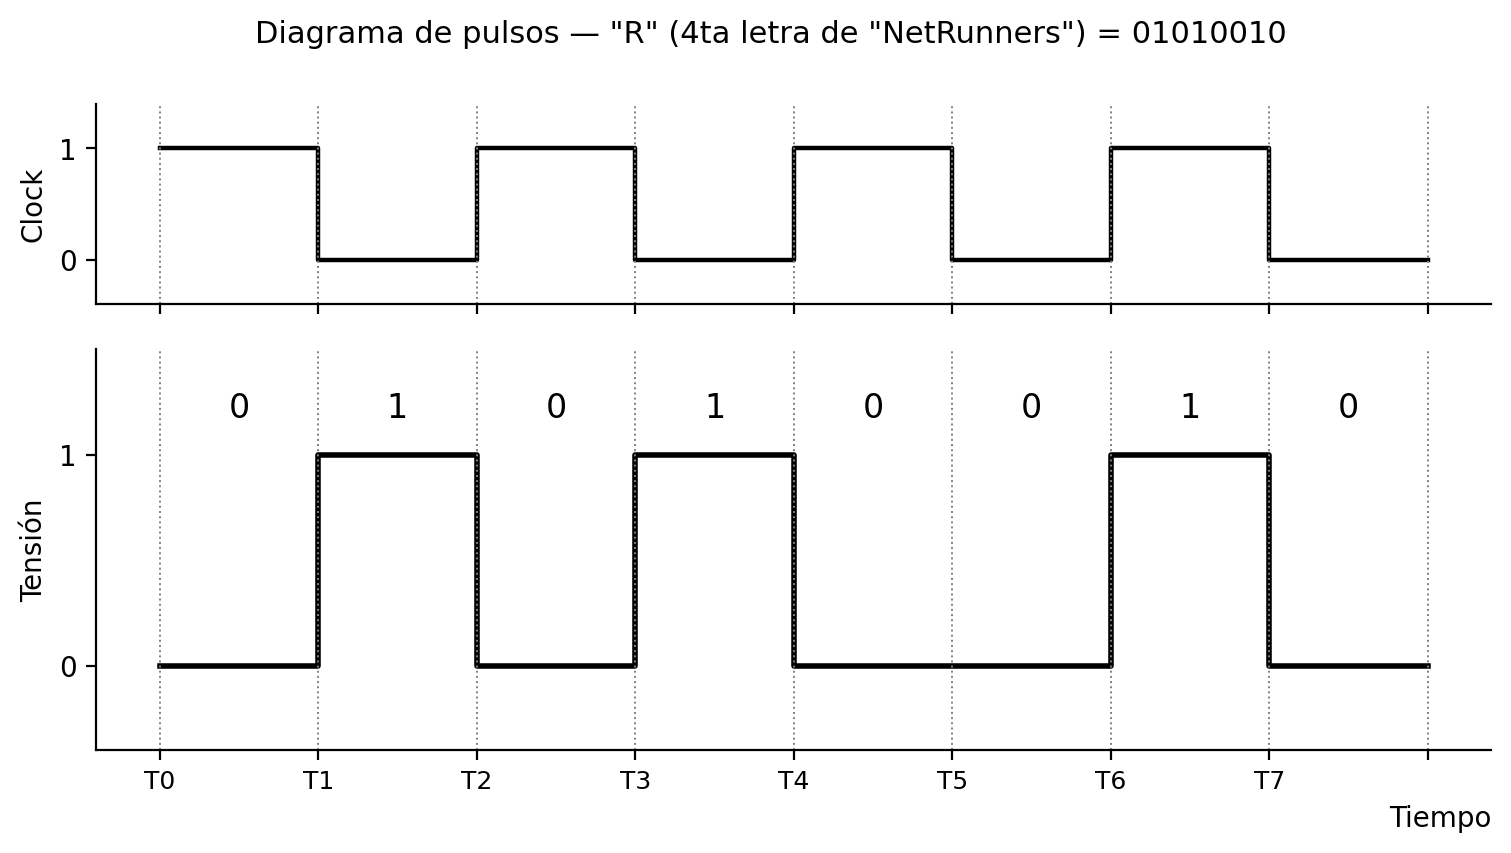
\includegraphics[width=0.8\textwidth]{2_c.png}
    \end{figure}

    \item Para poder dar una lectura confiable, idealmente hay que medir la señal en el punto medio entre $T3$ y $T4$, para que el margen de error por un posible desfasaje no sea grave.
\end{enumerate}

\section{}

\begin{enumerate}[label=\alph*.]
    \item Observando el gráfico, claramente la técnica de modulación utilizada es \textbf{“Modulación de Fase”} o \textbf{PSK} (\textit{Phase Shift Keying}), ya que vemos que lo que varía al cambiar el dato es dónde arranca la onda (cambia la fase).

    \item Siguiendo el gráfico de ejemplo, la nueva señal para la secuencia quedaría representada mediante el gráfico correspondiente.
    
    \begin{figure}[H]
        \centering
        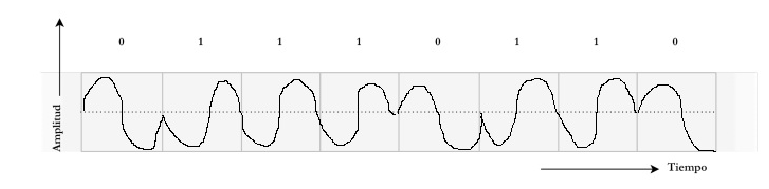
\includegraphics[width=0.8\textwidth]{3_b.png}
    \end{figure}

    \item Dentro de las técnicas PSK encontramos:
    \begin{itemize}
        \item \textbf{BPSK} (\textit{Binary Phase Shift Keying}): Representada en el gráfico anterior, usa sólo dos fases ($0^\circ$ y $180^\circ$) y transmite $1\text{ bit}$ por símbolo.
        \item \textbf{QPSK} (\textit{Quadrature Phase Shift Keying}): Usa 4 fases separadas ($0^\circ, 90^\circ, 180^\circ \text{ y } 270^\circ$) y codifica $2\text{ bits}$ por símbolo, duplicando la velocidad de datos sin requerir más ancho de banda.
        \item \textbf{PSK M-ario} (8-PSK, 16-PSK, etc.): Emplea un número $M$ de estados de fase y permite agrupar más bits por símbolo.
    \end{itemize}

    \item El \textbf{BER} (\textit{Bit Error Rate}) es una métrica que muestra los bits mal recibidos frente a los bits totales transmitidos, debido a que en transmisiones reales el ruido está siempre presente y hace que algunos bits sean recibidos incorrectamente.
    
    Teniendo esto en mente, la técnica que ofrece mejores prestaciones (mayor robustez contra el ruido) es \textbf{BPSK} (\textit{Binary Phase Shift Keying}). Esto se debe a que, al usar únicamente dos estados de fase separados por $180^\circ$, existe el mayor margen de tolerancia ante interferencias antes de cometer un error de interpretación, reduciendo así el BER y el número de puntos en el plano al ser de un orden inferior ($M = 2$).
\end{enumerate}

\section{Simulación y Conectividad}

\begin{figure}[H]
    \centering
    \textbf{Topología de Red:}\\[0.2cm]
    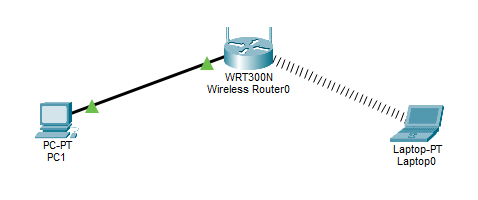
\includegraphics[width=0.75\textwidth]{4_a1.png}
\end{figure}

\begin{figure}[H]
    \centering
    \textbf{PC:}\\[0.2cm]
    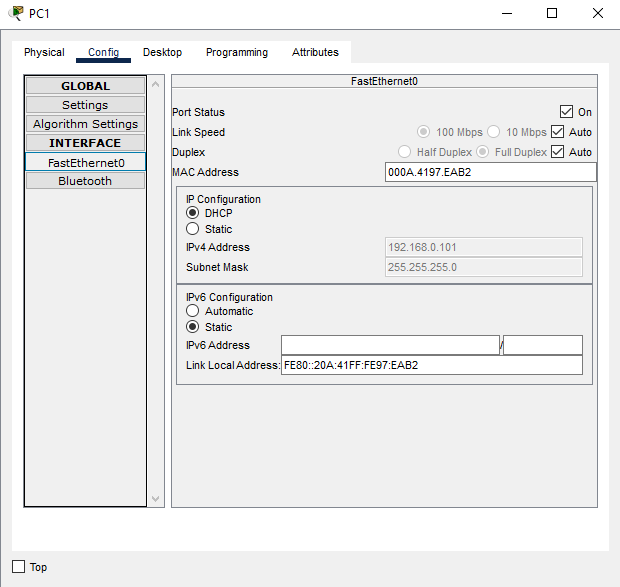
\includegraphics[width=0.65\textwidth]{4_a2.png}
\end{figure}

\begin{figure}[H]
    \centering
    \textbf{Laptop0:}\\[0.2cm]
    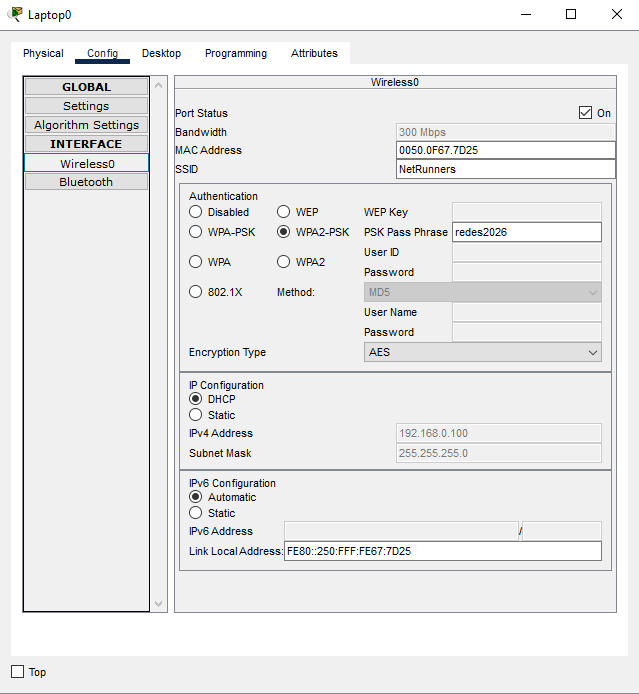
\includegraphics[width=0.65\textwidth]{4_a3.png}
\end{figure}

\begin{enumerate}[label=\alph*.]
    \setcounter{enumi}{2}
    \item \textbf{Análisis de configuración del Router:}
    \begin{itemize}
        \item \textbf{¿En qué frecuencia opera?} Opera exactamente en la frecuencia de $2.412 \text{ GHz}$.
        \item \textbf{¿A qué región del espectro electromagnético corresponde?} Corresponde a la región de las microondas.
        \item \textbf{¿En qué banda opera?} Opera en la banda de $2.4 \text{ GHz}$, la cual se clasifica dentro del rango de Frecuencias Ultra Altas (\textbf{UHF}).
    \end{itemize}

    \setcounter{enumi}{6}
    \item \textbf{Conectividad Laptop0 $\rightarrow$ PC:}
    
    \begin{figure}[H]
        \centering
        \textbf{Prueba Ping:}\\[0.2cm]
        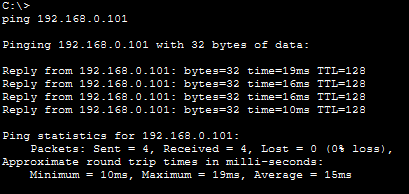
\includegraphics[width=0.75\textwidth]{4_g1.png}
    \end{figure}

    \begin{figure}[H]
        \centering
        \textbf{Prueba Tracert:}\\[0.2cm]
        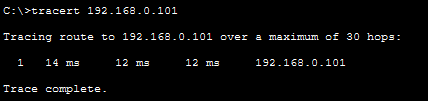
\includegraphics[width=0.75\textwidth]{4_g2.png}
    \end{figure}

    \item \textbf{Conexión Laptop0 $\rightarrow$ Laptop1:}
    Se ubicó la Laptop1 en dos coordenadas distintas respecto a la red Wi-Fi. Se ejecutó una prueba de conectividad (\texttt{ping}) hacia la Laptop0 para medir alcance, tiempos de respuesta y tasa de pérdida de paquetes.

    \begin{figure}[H]
        \centering
        \textbf{Ubicación Dentro de Cobertura:}\\[0.2cm]
        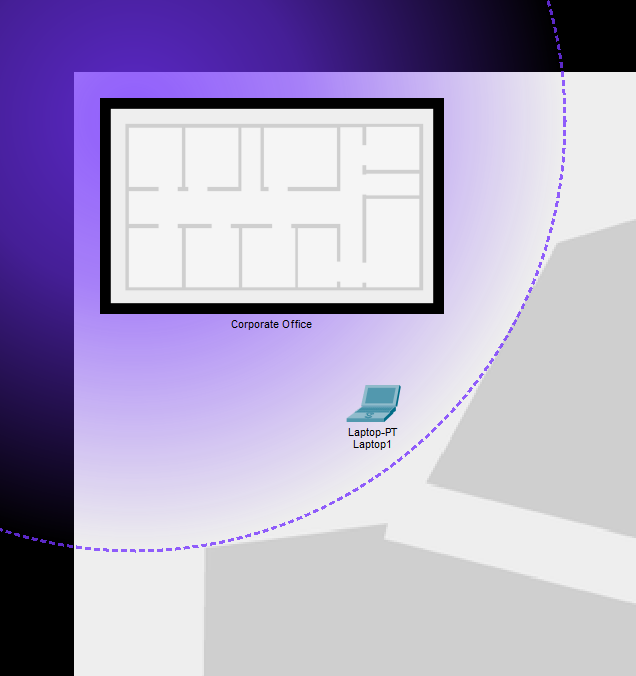
\includegraphics[width=0.65\textwidth]{4_h1.png}
    \end{figure}

    \begin{figure}[H]
        \centering
        \textbf{Ping - Dentro de Cobertura:}\\[0.2cm]
        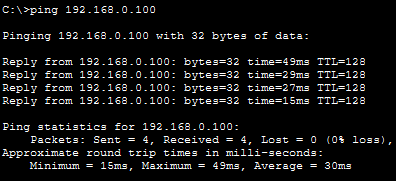
\includegraphics[width=0.7\textwidth]{4_h2.png}
    \end{figure}

    \begin{figure}[H]
        \centering
        \textbf{Ubicación Fuera de Cobertura:}\\[0.2cm]
        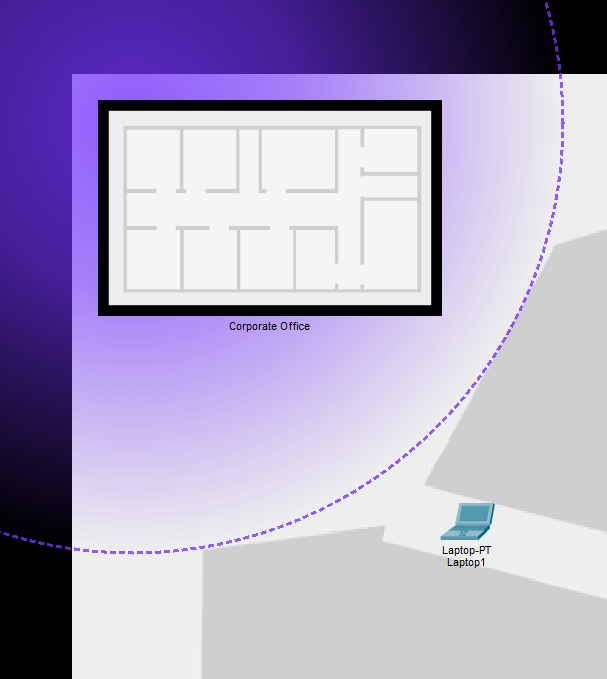
\includegraphics[width=0.65\textwidth]{4_h3.png}
    \end{figure}

    \begin{figure}[H]
        \centering
        \textbf{Ping - Fuera de Cobertura:}\\[0.2cm]
        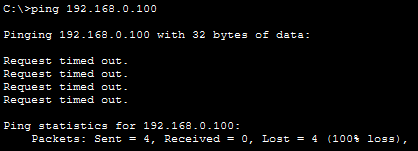
\includegraphics[width=0.7\textwidth]{4_h4.png}
    \end{figure}

    \begin{table}[H]
        \centering
        \caption{Pruebas de conectividad según cobertura Wi-Fi}
        \vspace{0.2cm}
        \begin{tabular}{l c c c}
            \toprule
            \textbf{Posición (Área)} & \textbf{IP} & \textbf{Paquetes (E/R/P)} & \textbf{Latencia (ms)} \\
            \midrule
            Dentro & 192.168.0.100 & 4/4/0 & 30 \\
            Fuera  & 192.168.0.100 & 4/0/4 & N/A \\
            \bottomrule
        \end{tabular}
    \end{table}

    \textbf{Conclusiones sobre lo medido:}
    \begin{itemize}
        \item \textbf{Comportamiento dentro del radio de cobertura:} Cuando la Laptop1 se encuentra dentro del área de alcance del punto de acceso (Router), la comunicación es completamente exitosa ($0\%$ de pérdida de paquetes). Se observa un tiempo promedio de respuesta (\textit{Round Trip Time} - RTT) de $30\text{ ms}$, lo que indica una latencia estable para un medio no guiado.
        \item \textbf{Efecto de la atenuación por distancia:} Al desplazar la Laptop1 fuera del radio de cobertura efectivo de la señal inalámbrica, los paquetes sufren una atenuación tal que la relación señal-ruido ($SNR$) impide mantener el enlace físico.
        \item \textbf{Resultado del agotamiento de tiempo:} Como consecuencia del punto anterior, la prueba finaliza con el error \textit{"Request timed out"} (tiempo de espera agotado) para el $100\%$ de los paquetes enviados ($4/0/4$), confirmando la pérdida total del canal de transmisión al sobrepasar el límite físico del medio.
    \end{itemize}
\end{enumerate}

\end{document}